%\documentclass[14pt, notes]{beamer}
\documentclass[14pt]{beamer}

%\usepackage{pgfpages}
%\setbeameroption{show notes}
%\setbeameroption{show notes on second screen=right}

%encoding
\usepackage[utf8]{inputenc}

%language
\usepackage[russian]{babel}
\usepackage{amsmath}
\usepackage{bm}
\usepackage{graphicx}
\usepackage{hyperref}
\graphicspath{{images/}}%путь к рисункам

\setbeamerfont{author in head/foot}{size=\small}
\setbeamerfont{title in head/foot}{size=\footnotesize}

\title[Моделирование динамики жидкости в сосудах]{Моделирование динамики жидкости в крупных кровеносных сосудах}
\date{\today}
\author[Долгов Д.А.]{Долгов Д.А.\\{\small Научный руководитель: Захаров Ю.Н.}}
\institute{Кемеровский Государственный Университет \\
    \vspace{0.7cm}
    \vspace{0.7cm}
} 
\usetheme[numbers, totalnumbers, minimal, nologo]{Statmod}
% Привычный шрифт для математических формул
\usefonttheme[onlymath]{serif}

\definecolor{statmodblue}{RGB}{100,10,30}
\definecolor{statmodsand}{RGB}{244,215,103}

\begin{document}
\maketitle

%description of the problem
\begin{frame}
\frametitle{Введение}
Рассмотрим задачу о течении крови внутри крупных сосудов с гибкими стенками и клапанами. Кровь будем моделировать как вязкую, несжимаемую двухкомпонентную жидкость (плазма + форменные элементы: эритроциты, лейкоциты, тромбоциты), стенки сосуда и лепестки клапанов - как поверхность заданной формы, обладающую определенной жесткостью.
\end{frame}

%description of the problem: schema
\begin{frame}
\frametitle{Введение}
    \begin{center}
        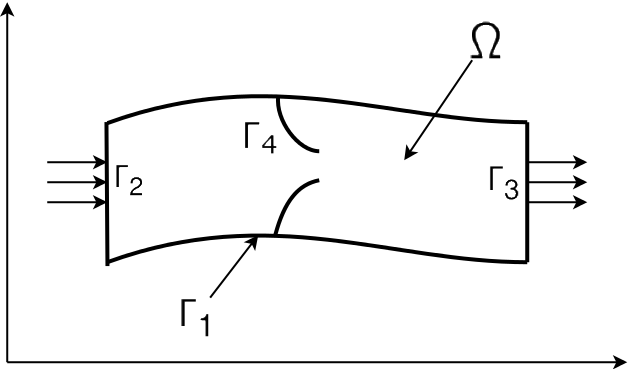
\includegraphics[width=9cm]{area.png}
    \end{center}
\end{frame}
\note{$\Gamma_1,\Gamma_4$ - гибкие стенки, $\Gamma_2,\Gamma_3$ - вход/выход}

% navier stokes equations
\begin{frame}
\frametitle{Моделирование течения}
Система уравнений Навье-Стокса:
\begin{gather}
    \label{eq:motion}
    \rho ( \frac{\partial u}{\partial t} + u \cdot \nabla u) = - \nabla p + \nabla \cdot \sigma + f\\
    \label{eq:continuity}
    \nabla \cdot u = 0 
\end{gather}
где $\sigma = \mu (\nabla u + (\nabla u)^{T})$, с начальными условиями
\begin{gather}
    u(x, y, z, t_0) = 0,\;p(x, y, z, t_0) = p_0
\end{gather}

\end{frame}
\note{Уравнения записаны в векторном виде, $\sigma$ - вязкий тензор напряжений}

% boundary
\begin{frame}
\frametitle{Условия на стенках}
\begin{itemize}
    \item на $\Gamma_1,\Gamma_4$ задаются условия прилипания
    \item на $\Gamma_2,\Gamma_3$ заданы значения давления $P_{int},P_{out}$
\end{itemize}

Помимо этого в каждой точке стенки определена поверхностная сила сопротивления деформации
\begin{equation*}
    \label{eq:define_boundary_force}
    F = F(x, y, z, t)
\end{equation*}

\end{frame}
\note{Условие прилипания в данном случае означает, что граница будет двигаться с той же скоростью, что и жидкость}

% concentration
\begin{frame}
\frametitle{Концентрация}
Уравнение для расчета концентрации примеси в жидкости:
\begin{gather}
    \label{eq:concentration}
    \frac{\partial c}{\partial t} + u \cdot \nabla c = D \triangle c
\end{gather}
где $D$ - коэффициент диффузии, с краевыми условиями на $\Gamma_1$
\begin{gather}
    \frac{\partial c}{\partial \vec{n}} = 0
\end{gather}

\end{frame}
\note{Эта часть еще в работе, нет четкого понимания с медицинской точки зрения, так что пока мы готовим общий подход, который в дальнейшем будем уточнять}

% concentration: dependencies
\begin{frame}
\frametitle{Концентрация}
Предполагается, что плотность и вязкость зависят от концентрации:
\begin{gather}
    \label{eq:concentration_viscosity}
    \mu = c (\mu_2 - \mu_1) + \mu_1\\
    \label{eq:concentration_density}
    \rho = c (\rho_2 - \rho_1) + \rho_1
\end{gather}

где $\mu_1, \mu_2, \rho_1, \rho_2$ - вязкости и плотности обоих компонент в начальный момент времени.
\end{frame}

% solve method 
\begin{frame}
\frametitle{Метод решения}
В соответствии с методом погруженной границы, будем рассматривать отдельно задачи вычисления параметров течения жидкости и параметров движения стенок сосуда и клапанов. Для этого введем в расчетной области сетки:
\begin{itemize}
    \item $\Omega = \Omega(x, y, z)$ - равномерная разнесенная сетка для расчета течения
    \item $\Gamma = \Gamma(q, r, s, t)$ - соответствует стенкам сосуда и клапанам в лагранжевых координатах
\end{itemize}

\end{frame}

% solve method: diagram
\begin{frame}
\frametitle{Метод решения}
    \begin{center}
        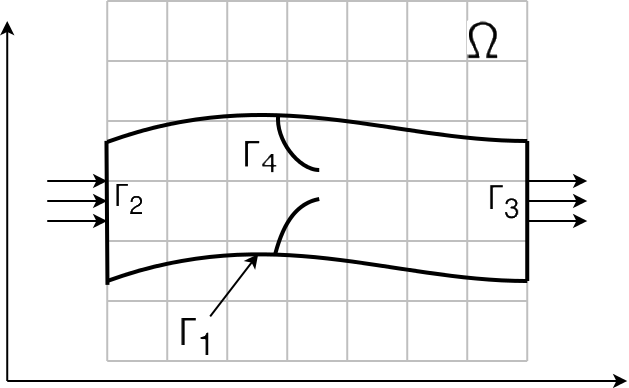
\includegraphics[width=9cm]{area_ibm.png}
    \end{center}
\end{frame}

% solve method: membranes nature
\begin{frame}
\frametitle{Метод решения}
Стенки сосуда и клапаны моделируются с помощью безмассовых (или с "нейтральной плавучестью" (neutrally buoyant)) фибр (коллагеновых фибр в случае сердечно-сосудистой системы), погруженных в жидкость.
\end{frame}

% solve method:immersed boundary
\begin{frame}
\frametitle{Взаимодействие}
В такой постановке необходимо добавить следующие уравнения, которые будут описывать взаимодействие погруженной границы и жидкости:
\begin{gather}
    \label{eq:ibm_velocity}
    \frac{\partial X}{\partial t} = \int_{\Omega} u \cdot \delta (x - X)\; dx\; dy\; dz \\
    \label{eq:ibm_force}
    f = \int_{\Gamma} F \cdot \delta (x - X)\; dq\; dr\; ds
\end{gather}
и условия прилипания
\begin{gather}
    \label{eq:no_slip}
    \frac{\partial X}{\partial t} (q, r, s, t) = u(X(q, r, s, t), t)
\end{gather}
\end{frame}
\note{Заглавные символы относятся к погруженной границе, обычные - к жидкости}

% solve method:additional equations for density, viscosity
\begin{frame}
\frametitle{Взаимодействие}
Для случая переменной плотности добавлять уравнениe:
\begin{gather}
    \label{eq:ibm_density}
    \rho = \int_{\Gamma} M \cdot \delta (x - X)\; dq\; dr\; ds
\end{gather}

В существующих работах [2] есть доказательство того, что $\frac{\partial \rho}{\partial t} + u \cdot \nabla \rho = 0$ есть следствие из \eqref{eq:continuity}, \eqref{eq:ibm_density}, \eqref{eq:ibm_velocity}

\end{frame}
\note{Пока не ясно насчет аналогичного уравнения для вязкости ($\mu = \int_{\Omega} M \cdot \delta (x - X)\; dq\; dr\; ds$) - видимо, оно требуется, судя из численного алгоритма, но во-первых, не ясно, как интерпретировать вязкость на границе, во-вторых, это явно не указано в теории. При этом т.к. в нашем случае плотность и вязкость зависят явно от концентрации, не ясно ли, можно ли заменить это уравнение на аналогичное для концентрации}

% solve method:note about concentration
\begin{frame}
\frametitle{Взаимодействие}
В текущей реализации краевые условия для концентрации задаются на $\Omega$ вместо $\Gamma_1$, что скорее всего дает меньшую точность. В существующих работах практически не встречается реализация подобных условий (см. [3]). Есть предположение, что этого можно добиться с помощью подхода, аналогичного для скорости.
\end{frame}

% solve method: algorithm 
\begin{frame}
\frametitle{Алгоритм решения}
\setbeamercolor{normal text}{fg=gray,bg=}
\setbeamercolor{alerted text}{fg=black,bg=}
\usebeamercolor{normal text}
    \begin{itemize}
        \item \alert<+>{Рассчитываем параметры течения в $\Omega(x, y, z)$, в частности векторное поле скорости}
        \item \alert<+>{С помощью полученной скорости вычислить скорость движения точек границы и ее деформацию}
        \item \alert<+>{На основе деформации $\Gamma(q, r, s, t)$ находим силу сопротивления $F(q, r, s, t)$}
        \item \alert<+>{С помощью $F(q, r, s, t)$ вычислить $f(x, y, z, t)$ для жидкости}
        \item \alert<+>{Перейти к новому временному слою с измененной $f(x, y, z, t)$}
    \end{itemize}
\end{frame}

% solve method:split scheme
\begin{frame}
\frametitle{Схема расщепления}
\begin{gather}
    \label{eq:split_first}
    \frac{u^* - u^n}{\triangle t} = - (u^n \cdot \nabla) u^n + \frac{1}{\rho} \nabla \sigma + f\\
    \label{eq:split_second}
    \rho \triangle p^{n+1} - (\nabla p \cdot \nabla p^{n+1}) = \frac{\rho^2 \nabla u^*}{\triangle t}\\
    \label{eq:split_third}
    \frac{u^{n+1} - u^*}{\triangle t} = - \frac{1}{\rho} \nabla p^{n+1}
\end{gather}
где $\nabla \sigma (u^n, \mu) = \mu \triangle u^n + (\nabla \mu \cdot \nabla) u^n + (\nabla \mu \cdot J_{u^n}) $
\end{frame}

% solve method:split algorithm 
\begin{frame}
\frametitle{Алгоритм решения}
\setbeamercolor{normal text}{fg=gray,bg=}
\setbeamercolor{alerted text}{fg=black,bg=}
\usebeamercolor{normal text}
    \begin{itemize}
        \item \alert<+>{Аппроксимируем уравнение \eqref{eq:split_first} с помощью схемы расщепления Дугласа-Рекфорда и решаем полученную систему методом прогонки}
        \item \alert<+>{Из уравнения \eqref{eq:split_second} методом бисопряженных градиентов определяем поле давления}
        \item \alert<+>{Восстанавливаем окончательное поле вектора скорости по явным формулам \eqref{eq:split_third}}
    \end{itemize}
\end{frame}

% solve method:ibm scheme
\begin{frame}
\frametitle{Алгоритм решения}
Интерполяция скорости на границу и распределение поверхностной силы деформации на точки жидкости:
\begin{gather}
    \label{eq:interpolation}
    U_n = \sum_{ijk}u_{ijk} \cdot D(x_{ijk} - x_n) h_{ijk}^3 \\
    \label{eq:spreading}
    f_{ijk} = \sum_n F_n \cdot D(x_{ijk} - x_n) h^2_n
\end{gather}

$D(x_n)$ соответствует $\delta(x - x_k)$, а $h_n$ - шаг сетки по погруженной границе.
\end{frame}

% solve method: force distribution scheme
\begin{frame}
\frametitle{Схема распределения силы деформации}
    \begin{center}
        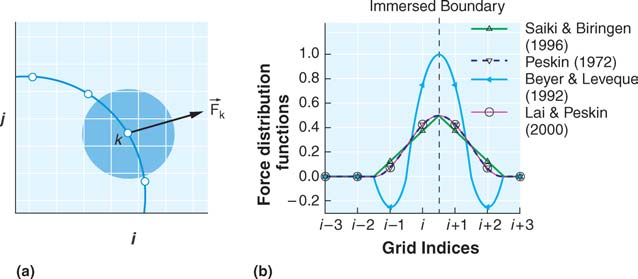
\includegraphics[width=11.5cm]{delta_function.png}
    \end{center}
\end{frame}

% solve method:boundary force, penalty method
\begin{frame}
\frametitle{Метод штрафов}
Сила находится исходя из смещения от начального положения:
\begin{gather}
    \label{eq:penalty_method}
    F_n = -k_n (q_n - q^{*}_n)
\end{gather}
где $F_n$ - проекция силы на одну из осей, для $(q, r, s) \in \Gamma$
\end{frame}

% solve method:boundary force, simple extension-compression and bendind resistance
\begin{frame}
\frametitle{"Наивный" метод расчета сил}
Сила состоит из силы сопротивления растяжению и скручиванию, и находится исходя из смещения относительно соседних точек:
\begin{gather}
    \label{eq:naive_extension}
    F^s_n =  k_s \sum_{m \ne n} \frac{d_{nm} - d^0_{nm}}{d_{nm}} \frac{x_n - x_m}{d_{nm}}
\end{gather}
где $F^s_n = F^s_n(X_1, X_2),\;X_{1,2} \in \Gamma$, а $d_{nm}$ - расстояние между точками
\end{frame}
\note{Деление на $d_{nm}$ - нормализация}

% solve method:boundary force, simple extension-compression and bendind resistance
\begin{frame}
\frametitle{"Наивный" метод расчета сил}
\begin{gather}
    \label{eq:naive_extension}
    F^b_n =  k_b \sum_{\substack{m \ne n\\l \ne n}} (\alpha_{mln} - \alpha^0_{mln}) \vec{n}_{ml}
\end{gather}
где $F^s_n = F^s_n(X_1, X_2, X_3),\;X_{1,2,3}(q, r, s) \in \Gamma$, \\
$\alpha_{mln}$ - угол, образованный тремя точками, \\
$\vec{n}_{ml}$ - единичный нормальный вектор
\end{frame}

% solve method:boundary force, strain energy
\begin{frame}
\frametitle{Расчет с помощью энергии деформации}
Каждой точке границы $(q, r, s)$ соответствует фибра, которую можно параметрически описать с помощью $s$ в виде $s \rightarrow X(q_0, r_0, s)$
\begin{gather}
    \label{eq:strain_energy}
    F =  \frac{\partial}{\partial s}(T \tau) + \frac{\partial^2}{\partial s^2} \Big( k \frac{\partial^2}{\partial s^2} X \Big)\\
    k = E \cdot I
\end{gather}
где $E$ - модуль Юнга, $I$ - момент инерции поперечного сечения, $T$ - напряжение фибры, $\tau$ - единичный тангенциальный вектор, касательный к фибре.
\end{frame}
\note{Модуль Юнга (и, как видимо, момент инерции поперечного сечения) - "инженерные" параметры, которые могут быть получены из эксперимента, $T$ - неясно, но, видимо, тоже зависит от модуля Юнга}

% totals and examples
\begin{frame}
\frametitle{Метод решения}
Данный метод разрабатывался с учетом применения в исследовании биологических систем, для которых подвижность и эластичность границ является важным фактором.
Он разделяет одну сложную задачу на три более простые - моделирование течения, моделирование состояния границы и их взаимодействие.
\end{frame}

% totals and examples
\begin{frame}
\frametitle{Метод решения}
Это позволяет применять мощные методы для решения каждой из задач. Помимо этого такой подход позволяет единообразно моделировать различные классы проблем, т.к. погруженная граница может иметь практически любую форму.
\end{frame}

% totals and examples
\begin{frame}
\frametitle{Метод решения}
Метод погруженной границы пока не реализован ни в одном из крупных CFD пакетов (такая работа начата только в OpenFOAM, но она находится на стадии обсуждения сообществом).
\end{frame}

% totals and examples
\begin{frame}
\frametitle{Работы других коллективов}
\begin{itemize}
    \item IBAMR (UNC McAllister Heart Institute)
    \item \href{run:video/valve\_flow\_side.avi}{Пример моделирования аортального клапана}
    \item \href{run:video/MV\_side.avi}{Расчет параметров хордового протеза для митрального клапана}
\end{itemize}
\end{frame}

% totals and examples
\begin{frame}
\frametitle{Примеры}
\begin{itemize}
    \item \href{run:video/cylinder1.avi}{Деформация стенок сосуда}
    \item \href{run:video/cylinder2.avi}{Аналогичный расчет на более мелкой сетке}
\end{itemize}
\end{frame}

% totals and examples
\begin{frame}
\frametitle{Примеры}
\begin{itemize}
    \item \href{run:video/source_in_vessel.avi}{Расчет распространения примеси}
    \item \href{run:video/thrombus_in_vessel.avi}{Размыв "тромба"}
\end{itemize}
\end{frame}

\begin{frame}
\frametitle{Дополнительная информация}
    \begin{itemize}
        \item Peskin C.S., Numerical Analysis of Blood Flow in the Heart// JCP 25,220-252, (1977)
        \item Peskin C.S., The immersed boundary method// Acta numerica, 1-39, (2002)
        \item Peskin C.S., Griffith B.E., Pilhwa L., The immersed boundary method for advection-electrodiffusion with implicit timestepping and local mesh refinement, Comput Phys, (2010)
        \item Kruger T., Introduction to the immersed boundary method, (2011)
    \end{itemize}
\end{frame}
\note{
    \begin{itemize}
        \item Основная работа "непрерывного метода" (journal of computational physic)
        \item Более полная и развернутая
        \item Хороший обзор (Annual Review of Fluid Mechanics)
        \item Обзор в диссертационной работе
        \item Больше практики, но со спецификой другого метода расчета (Lattice Boltzmann method)
    \end{itemize}
}

\end{document}
